\documentclass[twocolumn]{article}

\usepackage[english]{babel} 

\usepackage[T1]{fontenc}
\usepackage{lmodern}
\usepackage[utf8]{inputenc}
\usepackage{graphicx}

\usepackage{ifthen}
\usepackage{xcolor}
\usepackage{tabu}
\usepackage{colortbl}
\usepackage{calc}

\usepackage{pifont}
\usepackage{forloop}
\usepackage[nomessages]{fp}
% Math

\usepackage{amsmath}
\usepackage{amssymb}
\usepackage{amsthm} 

\newtheoremstyle{break}
   {\topsep}{\topsep}%
   {\itshape}{}%
   {\bfseries}{}%
   {\newline}
   {\thmname{#1}\thmnumber{\@ifnotempty{#1}{ }\@upn{#2}}%
    \thmnote{ {\bfseries(#3)}}}% 
    
\newtheorem{definition}{Definition}

\usepackage[parfill]{parskip}
%\usepackage[onehalfspacing]{setspace}
\usepackage{newclude}

\newcounter{starnumber}
\newcommand{\stars}[1]{
  \forloop{starnumber}{1}{\value{starnumber} < 6}{
    \ifthenelse{#1 < \value{starnumber}}{\ding{73}}{\ding{72}}%
  }
}


%\usepackage[sortcites=true, style=authoryear,natbib=true]{biblatex}
\usepackage{biblatex}
\bibliography{bibliography}

%Autornamen in Bibliography fett
%\AtBeginBibliography{\renewcommand*{\mkbibnamelast }[1]{\textbf{#1}}}
%\AtBeginBibliography{\renewcommand*{\mkbibnamefirst }[1]{\textbf{#1}}}

%\makeindex

\title{Development of a educational and sustainable robotic platform for children and adults}
\date{\today}
\author{Sebastian Muszytowski \\Baden-Wuerttemberg Cooperative State University Mannheim }

\begin{document}

\twocolumn[
        \maketitle
        \begin{@twocolumnfalse}
        \maketitle
        \end{@twocolumnfalse}
]


\section{Introduction}
Getting children in touch with technology is important in todays technologically advanced society. In schools technology (specifically electrical engineering and programming) is often taught using robots. Robots are well suited for children since they allow interaction with the reality in contrast to arbitrary technology related exercises such as programming execises which doesn't affect the real world.\newline 
Since schools are required to save money, robots used for teaching stay property of the schools. Therefore children usually cannot take the robot home to work with it. In addition modification of robot is usually not permitted which reduces potential learning experiences. Giving students the full control over all possibilities of the robot requires them to own the robot. This requires to robot to be cheap, extendable and suitable for educational purposes.\newline
The development of a robot plattform for educational purpose requires requirement engineering, market research and evaluation of robots which are already used in education. Once the research is completed a new robot plattform can be constructed taking the research results into account.
\section{Requirement Analysis / Project Goals}
The target user group of the robot are mainly children and adults with very little or no experience in electrical engineering and programming. Teaching the knowledge requires a platform which is designed to be educational. Therefore it has to comply with several requirements which affect technical aspects as well as social aspects.
The following lists describes the basic requirements on which existing platforms can be assessed. The assessent critera can also be used to make decisions when developing a new platform.
\begin{description}
\item[Affordable] \hfill \\ The robot platform must be affordable for everyone. Especially when the robot is used in schools every child should own the robot to increase the possibilities to modify and extend it. Robots which stay property of a school may result in social problems since socially disadvantaged children cannot afford their own robot whereas socially advantaged children can. A considerable price tag for a educational robot is the educational budget for a wellfare recipient which is 100 Euro per year in Germany as defined defined in SGB II §28 (as of the 07.05.2013).
\item[Educational] \hfill \\ Documentation, learning materials and suggestions for lessons are needed to teach the usage of the robot. The robot should be designed to teach both electrical engineering as well as programming. This can be realized by having exercises specific to the topic e.g. by soldering the robot first with programming afterwards. By using strategies like Poka-yoke (mistake proofing) the platform becomes more robust and therefore can prevent frustration.
\item[Sustainable] \hfill \\ Sustainability is an environmental issue which should be taken into account. Sustainability includes serveral aspects such as the choice of materials, their durability and the repairability. It is a huge bonus if materials are environment-friendly and produced in a socially acceptable manner. If the robot can be easily repaired or interchanged using household or easy to get items the robot can be considered sustainable. 
\item[Extendable] \hfill \\ Extendabilitiy enables the robot to adapt to new tasks. Interchangeable sensors and actuators are the key to a flexible plattform. The plattform should provide some unused microcontroller pins dedicated to extensions. Those pins should be mapped onto easy accessible pins which require no soldering.  
\item[Open-Source] \hfill \\ Open-Source products can be easily modified, extended and remixed into new, continously improved, products. Schematics, build-instructions and specifications should be accessible under a permissive open-source license. 
\end{description}


\section{State of the Art}
The development of a new robot platform requires the assessment of current robotic platforms using the requirements developed. In focus of the assessment are popular robot platforms which are either actively used in schools or developed with education in mind. All of the platforms are independently developed and focus on different ideas. 

Assement criterias are evaluated using a rating system which allows values between zero and five where higher values are better. Each value is represented using stars for better overview. Detailed description of each rating is explained below.

\begin{description}
\item[\stars{5}] \hfill \\The evaluated aspect fully complies with the assessment critera and adds additional functionality which exceeds expectations. 
\item[\stars{4}] \hfill \\The evaluated aspect fully complies with the assessment critera. Mentioned properties may have minor restraints which do not affect the overall quality/functionality of the system.
\item[\stars{3}] \hfill \\The evaluated aspect complies with most of the assessment critera. The evaluation shows that some minor and/or major restraints exist which may affect the overall quality/functionality.
\item[\stars{2}] \hfill \\The evaluated aspect mets the assessment critera partially but shows severe restraints affecting the overall quality/functionality.
\item[\stars{1}] \hfill \\The evaluated aspect contains the rudiments of the assessment critera.
\item[\stars{0}] \hfill \\The evaluated aspect does not met the assessment critera in any way. 
\end{description}

\subsection{Asuro}
\begin{figure}[h!]
  \centering
  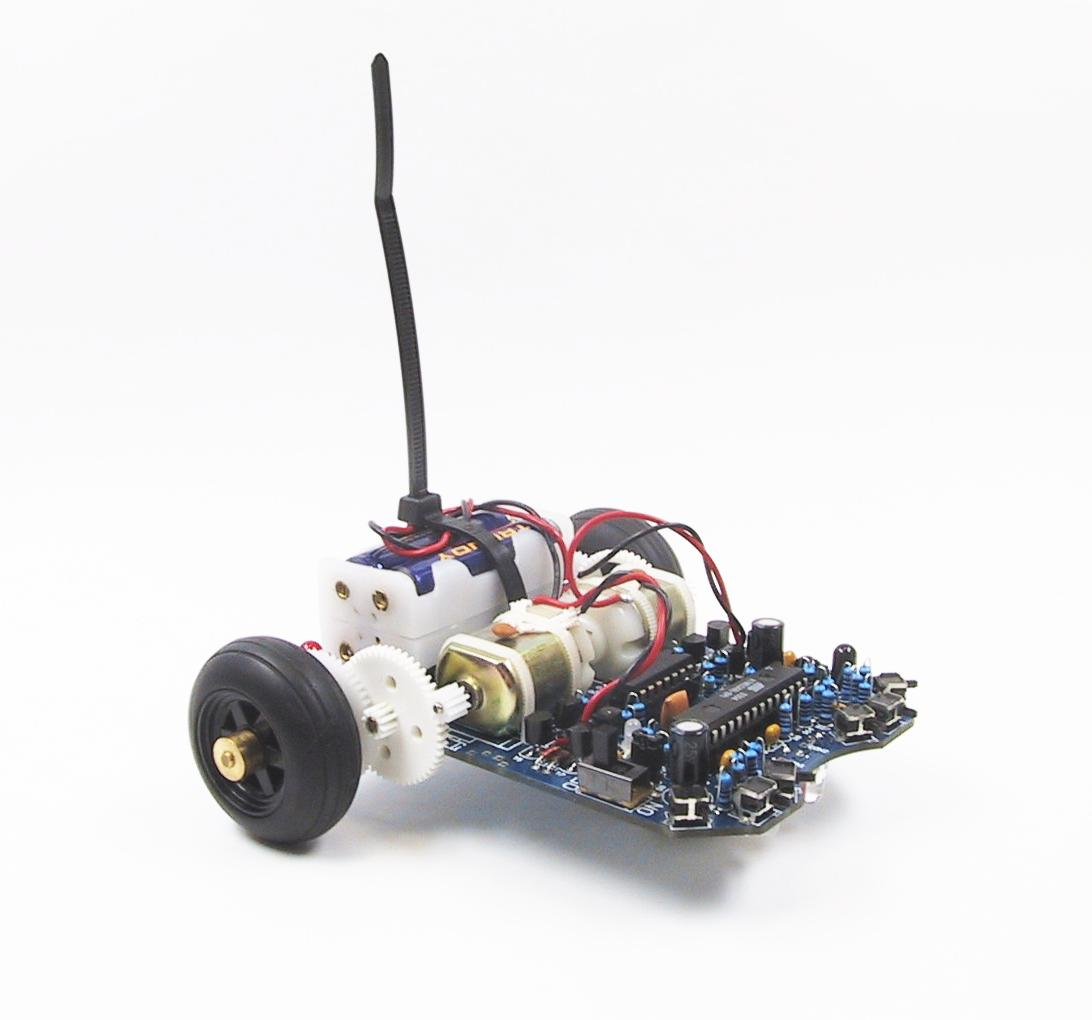
\includegraphics[width=0.5\textwidth]{images/asuro.jpg}
  \caption{Picture of the Asuro (CC-BY-SA Robin Gruber)}
\end{figure}

The Asuro robot is developed by the German Aerospace Center (Deutsches Zentrum für Luft- und Raumfahrt e.V.) in cooperation with Arexx Engineering focussed on edcuational use. Asuros development started in 2004 and is now discontinued. The robot is shipped as a do-it-yourself kit and requires about eight hours build time for a novice. 

Asuro features an eight bit Atmel ATmega8L microcontroller with eight kilobytes of flash memory, 512 bytes of electrical eraseable programmable read only memory (short EEPROM) and one kilobytes of static random-access memory (short SRAM). One kilobyte of flash is used for the bootloader which results in seven kilobytes of flash usable for user programs.

Interaction with the environment is realized using two DC motors which can be controlled individually in terms of direction and speed. The robot is stabilized using a half table-tennis ball mounted at the bottom of the robot. Four LEDs are used for displaying the status of the asuro. The whole system is powered by four AAA batteries or rechargable batteries mounted in a 2x2 battery case. 

Asuro can sense its environment using different sensors such as two photodiodes which can be used for line-following tasks, six push buttons to detect objects in front of Asuro and two photoelectric sensors to determine the rotation speed of each of Asuros wheels.


\subsection{Arduino Robot}
\begin{figure}[h!]
  \centering
  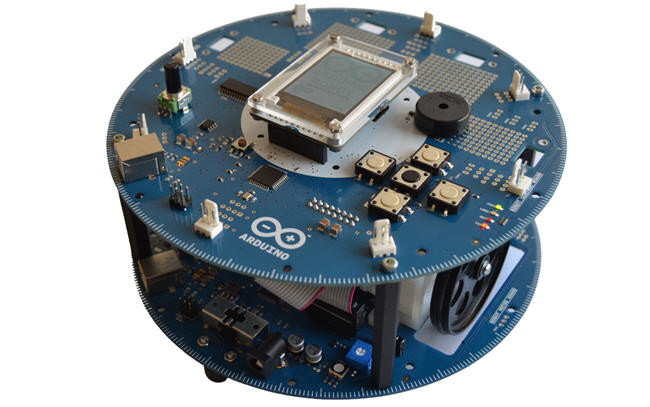
\includegraphics[width=0.5\textwidth]{images/arduinorobot.jpg}
  \caption{Picture of the Arduino Robot}
\end{figure}

The Arduino Robot is the first robot created by the arduino foundation. It comes preassembled and contains two microcontrollers 
\subsection{Lego Mindstorms}
\begin{figure}[h!]
  \centering
  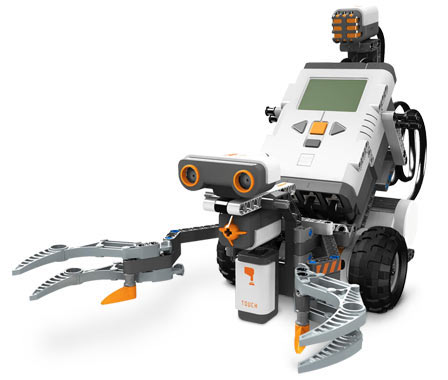
\includegraphics[width=0.5\textwidth]{images/mindstorms.jpg}
  \caption{Picture of the Lego Mindstorms NXT (from http://www.devoxx.com/)}
\end{figure}
\subsection{Thymio II}
\begin{figure}[h!]
  \centering
  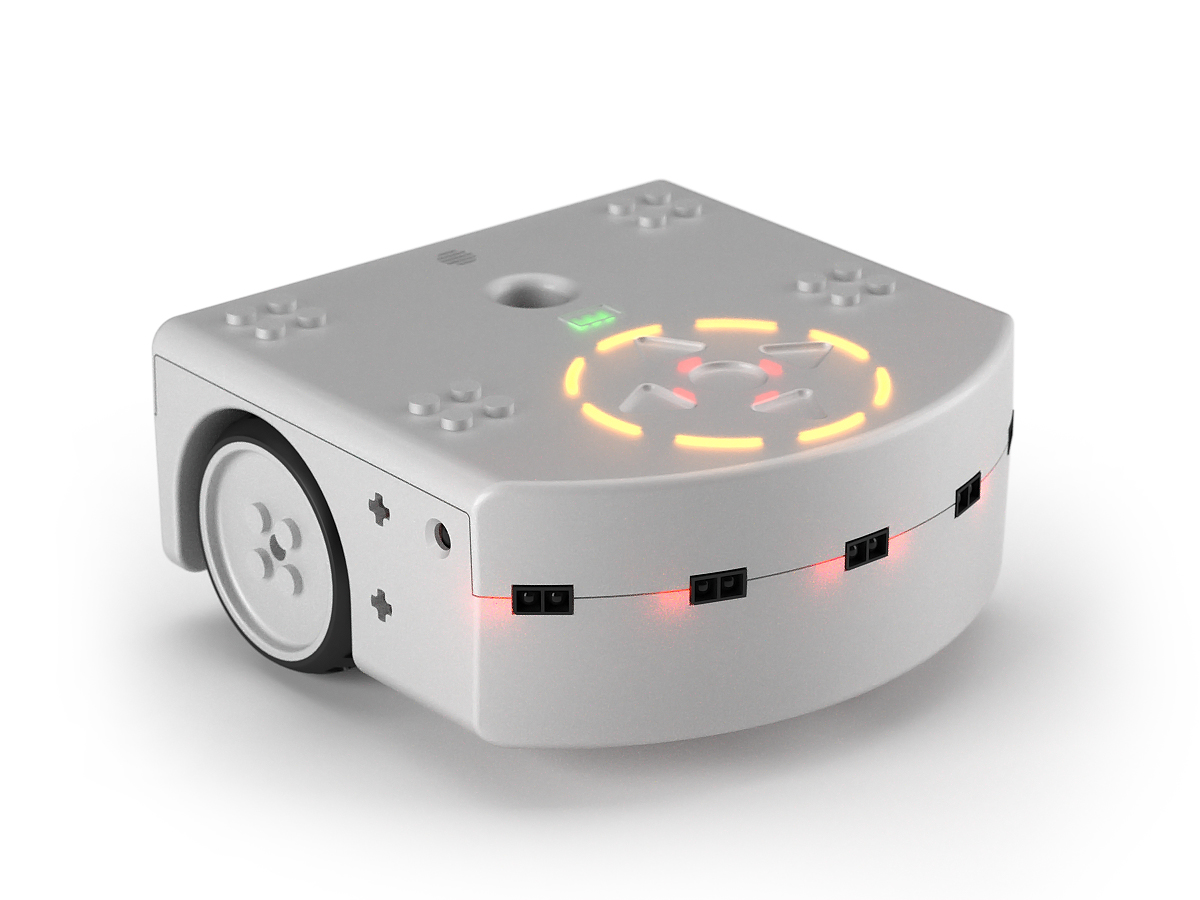
\includegraphics[width=0.5\textwidth]{images/thymioii.jpg}
  \caption{Picture of the Thymio II (from https://aseba.wikidot.com/en:thymio)}
\end{figure}


\section{Case studies}
A robot is built using parts and modules which can be grouped into functional groups like movement, sensors or communication. The goal of each functional group can be achieved in various ways which have to be evaluated using the requirements used in the evaluation of other robot platforms. The difficulty in the evaluation process are dependencies between different modules, e.g. when a sensor has special power requirements. 
\subsection{Movement}
Movement is the most important feature since it allows interaction with the robots environment. In contrast to a stationary robot a moving robot can interact with a wider area but requires battery power. Different approaches for robot movement exist which will be part of critical evaluation.
\subsubsection{Wheels}
Wheeled robots are common since their mechanic principle is rather simple. Typically robots have two wheels and a ball caster which prevents the robot from falling over. A ball caster acts as a third undirected wheel with reduced friction. Using wheels a robot can be moved in all directions.
\paragraph{Wheeled with two DC motors}
DC motors can be used to drive the wheels. To allow the control of direction (forward and backward) a so called H bridge is often used. Two H bridges can be combined to allow the robot to move right/left as well. 
\begin{figure}[h!]
  \centering
  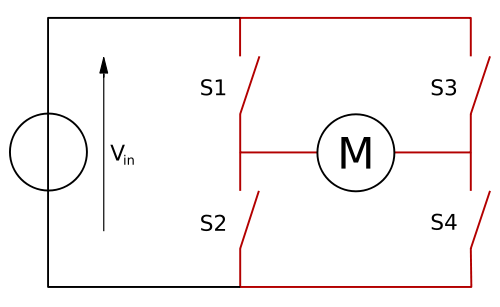
\includegraphics[width=0.5\textwidth]{images/hbridge.png}
  \caption{Basic schematic of a H-bridge (CC-BY-SA Cyril Buttay)}
\end{figure}
\paragraph{Wheeled with two Stepper motors}
Stepper motors are slightly modified DC motors. In stepper motors the full rotation is divided into a number of equal steps which can be separately controlled. The motor can step forward, backward or hold the current position with huge torque. Stepper motors are usually shipped within a gear box which reduces steps much further to gain higher precision and torque. 
These motors can be driven by a dual H bridge, a stepper driver or by using generic Input/Output pins in combination with a darlington array to reduce the current on the I/O pin. 

Stepper motors start at 2.95USD (in China) up to 4.95USD (in the USA\footnote{http://www.adafruit.com/products/858}). Two stepper motors are needed to drive the robot. To reduce the cost a ULN2803 darlington array with eight outputs can be used in combination with a eight bit shift-register (74HC595) to control the movement. This solution has a price tag of 2*2.95USD (steppers) plus 0.9USD (ULN2803) plus 0.9USD (74HC595) rendering a total cost of 8USD. Another advantage beneath the low costs are the parts itself. The afore mentioned shift register and darlington array are standard parts which come in beginner friendlly easy to solder SMD packages. 

The alternative solution is to use a stepper motor driver like Toshibas TB6612FNG which can drive either two DC motors or a single stepper motor. With a price of 3USD it is rather costly since two driver chips are needed for two stepper motors.

\paragraph{Omniwheels}

\paragraph{Comparison}


\subsubsection{Legs}
Bipod
Qadropod
Hexapod

\subsection{Sensors}
\subsection{Communication}
\subsection{Microcontroller}
\subsection{Power Supply}

\section{Robot Construction}



\nocite{*}
\printbibliography
\addcontentsline{toc}{part}{References}
\end{document}
